% !TEX root = team-report.tex
% ERA-Großpraktikum: Team Bericht -- Organisatorisches

\section{Organisatorisches}
\label{team:orga}

Dieses Kapitel behandelt die ``Logistik'' hinter der Entstehung von \erasim{} und
beschreibt, welche Strategie wir als Gruppe bei der Entwicklung des Simulators
befolgt haben. Sektion \ref{team:orga-structure} skizziert die Struktur und
Hierarchie der Gruppe, Sektion \ref{team:orga-plan} diskutiert den initialen und
letztendlichen Zeitplan für die Entwicklung und Abschnitt
\ref{team:orga-workflow} schildert schlussendlich unseren Workflow.

\subsection{Struktur}
\label{team:orga-structure}

Die Mannschaft hinter der Entwicklung des \erasim{} Simulators bestand anfangs aus
12 und schlussendlich aus 10 Studierenden. Das Team hat sich schon früh in
verschiedene, thematisch abgeschlossene Untergruppen aufgeteilt um die
Bearbeitung der zahlreichen und vielfältigen Aufgaben effektiver zu gestalten.
Des Weiteren wurde aus der Mannschaft ein Mitglied als Projektleiter bestimmt um
die Entwicklung des Simulators zu koordinieren, als Ansprechperson für
Projektbetreuer zu dienen sowie auch bestimmte infrastrukturelle Entscheidungen, wie die Nutzung des Online-Test-Servers \emph{Travis}, zu nehmen und diese zu realisieren.

Die Bestimmung der einzelnen Untergruppen und Aufteilung der Mannschaft in diese
wurde während einem der allerersten Treffen vollzogen und hat sich letztendlich
als eine der wichtigsten und besten ``Design-Entscheidungen'' für die effektive
Verwirklichung des Simulators herausgestellt. Konkret waren diese Untergruppen
\emph{Arch, Core, Parser} und \emph{GUI} genannt. Jede Gruppe bestand aus zwei
bis drei Mitgliedern und behandelte einen grundlegenden Aspekt der Entwicklung.
Genauer befasste sich

\begin{itemize}
  \item \textbf{Arch}, mit der Abstraktion und Beschreibung von allgemeinen Befehlssätzen (ISAs) sowie der konkreten Implementierung der RISC-V ISA;
  \item \textbf{Core}, mit architekturunabhängigen Implementierung eines Speichermodells sowie der Verbindung der Schnittstellten sämtlicher Module;
  \item \textbf{Parser}, mit der syntaktischen Beschreibung eines RISC-V Assemblerdialekts sowie Implementierung eines Codeinterpreters und
  \item \textbf{GUI}, mit der Entwicklung der grafischen Benutzeroberfläche des Simulators.
\end{itemize}

Die Aufteilung in diese Untergruppen hat es uns erlaubt, uns jeweils thematisch
auf einen Aspekt der Simulatorentwicklung zu fokussieren, Expertenwissen
innerhalb jeden Gebiets anzuhäufen und auszutauschen sowie Aufgaben effektiv zu
verteilen. Während der initialen Strukturierung des Teams hatten wir uns auch
überlegt, einen Repräsentanten aus jeder Untergruppe zu wählen. Da die Gruppe zu
Beginn mit 12 Personen eine nicht unbeachtliche Größe hatte, war diese
Überlegung durchaus sinnvoll. Um die Hierarchie jedoch nicht unnötig zu erhöhen,
haben wir uns letztendlich dagegen entschieden und nur einen Leiter für die
gesamte Gruppe, nicht aber jede Untergruppe gewählt. Dies hat sich als
vollkommen plausible Entscheidung herausgestellt.

Der Gruppenleiter wurde noch im Mai 2016 demokratisch bestimmt. Hierbei standen
zwei selbsternannte Kandidaten, Daniel Riedel und Peter Goldsborough, zur Wahl.
Letzterer wurde schließlich zum Leiter gewählt.

\subsection{Planung}
\label{team:orga-plan}

Die meisten Unternehmungen in der Arbeitswelt und darüber hinaus, für welche man
sich Erfolg wünscht, sind von drei essentiellen Grundbausteinen geprägt: eine
Vision für das Endergebnis; einem handfesten Plan, wie man diese Vision
verwirklichen möchte sowie letztendlich die notwendige Tugend und Investition an
Zeit, um den Plan zu befolgen und die Vision zu realisieren. Diese Sektion
beschreibt, welche Ausprägung wir den ersten beiden Sektionen gegeben haben.

\subsubsection{Die Vision}
\label{team:orga-plan-vision}

In den ersten sechs bis acht Wochen des Großpraktikumszeitraums beschäftigte
sich die Gruppe mit der Ausarbeitung eines groben Grundrisses für die
Architektur des Simulators, mit der Angewöhnung an die notwendigen Technologien
für die Implementierung sowie mit der Definition einer Vision und eines
Zeitplanes. Die Vision war primär von zwei Quellen beeinflusst. Zum einen waren
dies unsere eigenen Erfahrungen als Studierende in der Vorlesung
\emph{Einführung in die Rechnerarchitektur} (ERA). Da jeder von uns gerade erst
in derselben Situation wie unsere zukünftigen Kunden gesessen hatte, konnten wir
natürlich leicht spezifizieren, was uns und unseren Kommilitonen beim Erlernen
der maschinennahen Programmierung und Assemblersprachen geholfen hätte. Zum
anderen hatten wir durch den bereits existierenden und von uns in ERA genutzten
Simulator \emph{Jasmin}\footnote{Jasmin wurde während eines vorherigen
Großpraktikums in einer obskuren Skriptingsprache, namens ``Java'', entwickelt.}
einen Referenzpunkt für die Entwicklung von \erasim{}. Wir konnten analysieren,
welche Aspekte von Jasmin uns geholfen hatten, konnten aber insbesondere auch
jene Features nennen, welche uns an Jasmin nicht gefielen und diese als Ziele
für \erasim{} festlegen. Die Überlegungen dieser ersten Phase verfestigten sich
schließlich in den folgenden langfristigen Zielen:

\begin{enumerate}
  \item Die Funktionen von \erasim{} sollten eine Übermenge jener von Jasmin
  sein. Das bedeutet, dass sämtliche Aufgaben aus früheren Zentralübungen,
  Klausuren und Tutorübungen in unserem Simulator ausführbar sein sollten,
  soweit diese in RISC-V übersetzbar sind.
  \item Der Simulator soll zwar primär für die Lehre gedacht, jedoch nicht durch
  diese beschränkt sein. Auch weitere Einsatzgebiete, wie die Forschung,
  sollten, zumindest durch Erweiterungen der Grundversion, offen bleiben. Eine
  Grundanforderung hierfür war es, echte RISC-V Programme ausführen zu können.
  \item Als Voraussetzung für (2) sollte der Simulator nicht \emph{zeilen}-,
  sondern \emph{address}basiert sein. Das bedeutet, dass Marken Addressen im
  Speicher und nicht Zeilen im Text referenzieren sollten. Hierfür müssten
  Instruktionen auch entsprechend in den Speicher assembliert werden.
  \item Als wohl wichtigste Eigenschaft sollte \erasim{}, im Vergleich zu
  \emph{Jasmin}, nicht nur für einen bestimtmen Befehlssatz wie x86 oder ARM
  implementiert sein, sondern für beliebige Architekturen erweiterbar bleiben.
\end{enumerate}

\subsubsection{Der Zeitplan}
\label{team:orga-plan-time}

Neben der Definition einer Vision füllten wir die erste Phase des
Entwicklungszeitraums mit der Ausarbeitung einer langfristigen \emph{Roadmap}
sowie einer kurzfristigen, kontinuierlichen Strategie für die Entwicklungsarbeit
über die nächsten sechs Monate. Wir befassten uns also mit allen Aspekten der
Zeitplanung unseres Projekt. Hierbei ließen wir uns insbesondere durch die in
der Industrie allgegenwärtigen \emph{agilen Methoden} leiten. Wir wollten also
auf Wasserfalldiagramme verzichten, die die Entwicklung bis ins kleinste Detail,
Schritt für Schritt, vorschreiben. Stattdessen fokussierten wir uns auf die
Bestimmung von monatlichen \emph{Meilensteinen} für jede Untergruppe und
einigten uns darauf, diese Meilensteine in zwei-wöchigen \emph{Sprints}
bewältigen zu wollen. Die vollständige Roadmap kann in der initialen
Spezifikation des Projekts gefunden werden. Eine komprimierte Version lautet:

\begin{itemize}
  \bolditem{Juni}: Definition und Realisierung des Architekturinterfaces, parsen einfacher Befehle und Dummy Versionen von Speichermodell sowie GUI.
  \bolditem{Juli}: Implementierung und Parsen sämtlicher arithmetischer Befehle, Fertigstellung des Speichermodells und Herstellung von Verbindungswegen zwischen sämtlichen Modulen.
  \bolditem{August \& September}: Assemblierung von Befehlen zur Darstellung im Speicher, Parsen von Direktiven, Marken und Konstanten sowie vollständige Verbindung zwischen GUI und Core.
  \bolditem{Oktober}: Entwicklung von Pseudoinstruktionen, Direktiven, Makros und Serialisierungslogik.
  \bolditem{November}: Fertigstellung der visuellen I/O Module und projektweite Fehlerbehebung.
  \bolditem{Dezember \& Januar} Dokumentation und Bericht.
\end{itemize}

Sektion \ref{team:orga-plan-anal} liefert nun eine Analyse unserer Erfolge und Misserfolge bezüglich der Einhaltung dieses Zeitplans sowie der Realisierung unserer Vision.

\subsubsection{Analyse und Diskussion}
\label{team:orga-plan-anal}

Im Vergleich zwischen dem von uns festgelegten Plan und der Manier, in welcher wir das Projekt tatsächlich bewältigt haben, lassen sich zwei grundlegende Beobachtungen treffen:
\vspace{-0.2cm}
\begin{enumerate}
  \item Aufgrund mehrerer Faktoren ist die Fertigstellung einzelner Meilensteine, vor allem gegen Ende der Arbeitszeit, von obigem Zeitplan merkbar abgewichen,
  \item Dennoch haben wir unsere Vision bis auf wenige Aspekte realisiert und ein vollständiges Produkt entwickeln und abliefern können.
\end{enumerate}

Zusammenfassend kann man sagen, dass wir zwar alle initial festgelegten
Meilensteine erreicht haben, jedoch nicht immer in den geplanten Zeiträumen.
Beispielsweise wurde das Speichermodell nicht wie vorgesehen bereits im Juli,
sondern erst im September fertiggestellt. Ebenso wurde die (korrekte)
Assemblierungslogik zur realitätsnahen Darstellung von Instruktionen im Speicher
im Dezember und nicht bereits im August vollendet. Auch verschob sich ein nicht
unbeachtlicher Teil der Entwicklung der GUI auf Dezember und Januar. Grafik
\ref{fig:commit-history} zeigt ein interpoliertes Histogramm der Commitzahlen
auf das GitHub Repository des Projekts, während Grafik \ref{fig:time-frame}
einen Eindruck über die Diskrepanz zwischen geplanter und tatsächlicher
Fertigstellung von Meilensteinen gibt.

Wir behaupten, dass sich unsere Verplanung bei manchen der Meilensteinen auf vier Ursachen zurückz uführen lässt: Mangel an Erfahrung und Einschätzungsvermögen

\begin{figure}[p!]
  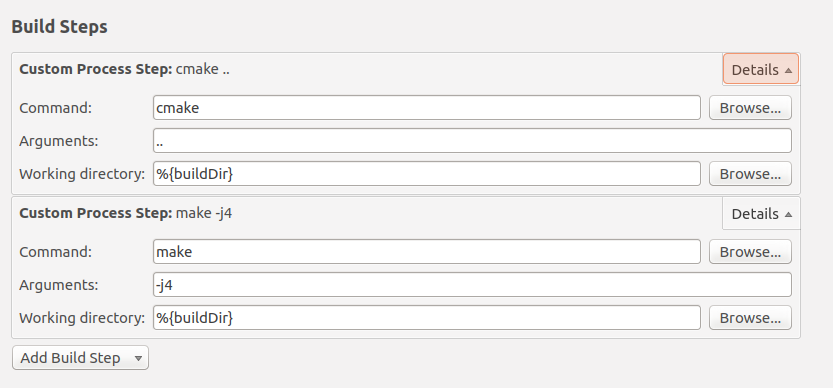
\includegraphics[scale=0.1]{figures/commit-history}
  \caption{Ein Histogramm der gesammelten Commitzahlen auf das GitHub Repository von \erasim{} während des Entwicklungszeitraumes.}
  \label{fig:commit-history}
\end{figure}

\begin{figure}[p!]
  \centering
  \begin{tikzpicture}[thick]
    \draw [|->] (0, 0) -- ++(16, 0);

    \newcount\x\relax
    \x=1\relax
    \foreach \month in {%
      Juni, Juli, August, September, Oktober, November, Dezember, Januar} {
      \draw (\x, 0.125) -- (\x, -0.125) node [below] {\small\month};
      \global\advance\x by 2\relax
    }

    \foreach \name/\planned/\actual/\y in {%
      Speichermodell/3/7/1.6,%
      Assemblierung/5/13/2.4,%
      RISC-V Instruktionen/6/3/3,%
      Direktiven und Makros/5/9/0.8,%
      Ausgabeanzeigen/11/15/3,%
      Verbindung aller Module/3/9/4%
    } {
      \path (\planned, \y) coordinate [fill, circle, inner sep=1.2pt] (p\name);
      \path (\actual, \y) coordinate [fill, circle, inner sep=1.2pt] (a\name);
      \ifnum\actual<\planned
        \newcommand{\arrowcolor}{NavyBlue}
      \else
      \newcommand{\arrowcolor}{Red}
      \fi
      \draw [->, very thick, dotted, \arrowcolor]
            (p\name) -- (a\name) node [above, midway]
            {\color{black}\small\name};
    }

  \end{tikzpicture}
  \caption{Diese Grafik beschreibt die Fertigstellung einer Auswahl an Meilensteinen. Hierbei werden für jeden Meilenstein der geplante und tatsächliche Zeitpunkt der Fertigstellung dargestellt. Pfeile verbinden diese Zeitpunkte, wobei Pfeilspitzen auf das tatsächliche Abschlussdatum zeigen.}
  \label{fig:time-frame}
\end{figure}

\subsection{Workflow}
\label{team:orga-workflow}

language
definitions of done
test driven
waffle
kommunikationsmittel
github
